\section{Results}

\subsection{Multihead DeePWAK learns sparse representations}

\begin{figure}
  %\begin{subfigure}[b]{0.5\textwidth}
  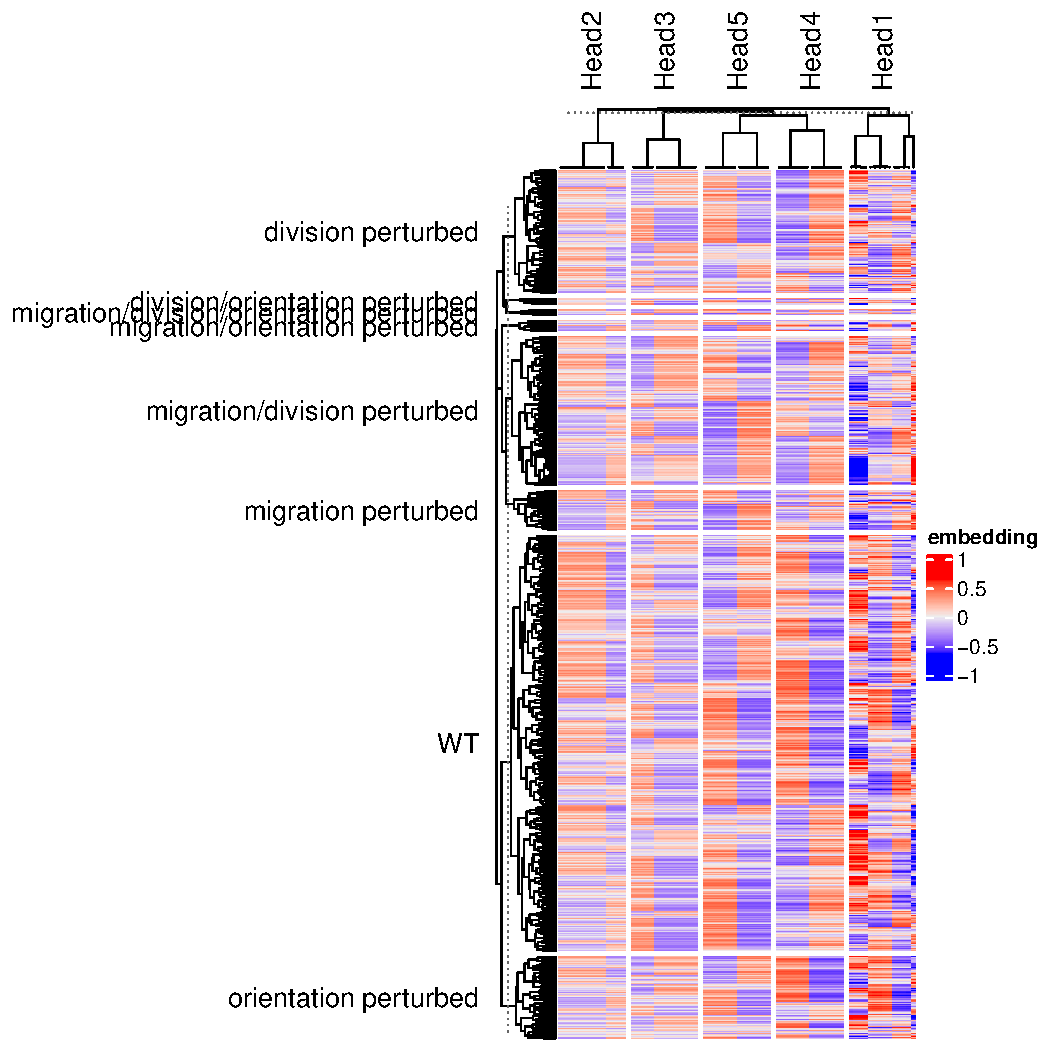
\includegraphics[width=\textwidth]{embeddings.pdf}
    \caption{DeePWAK learns sparse embedding values. }
    \label{fig:}
\end{figure}

    
\begin{figure}
  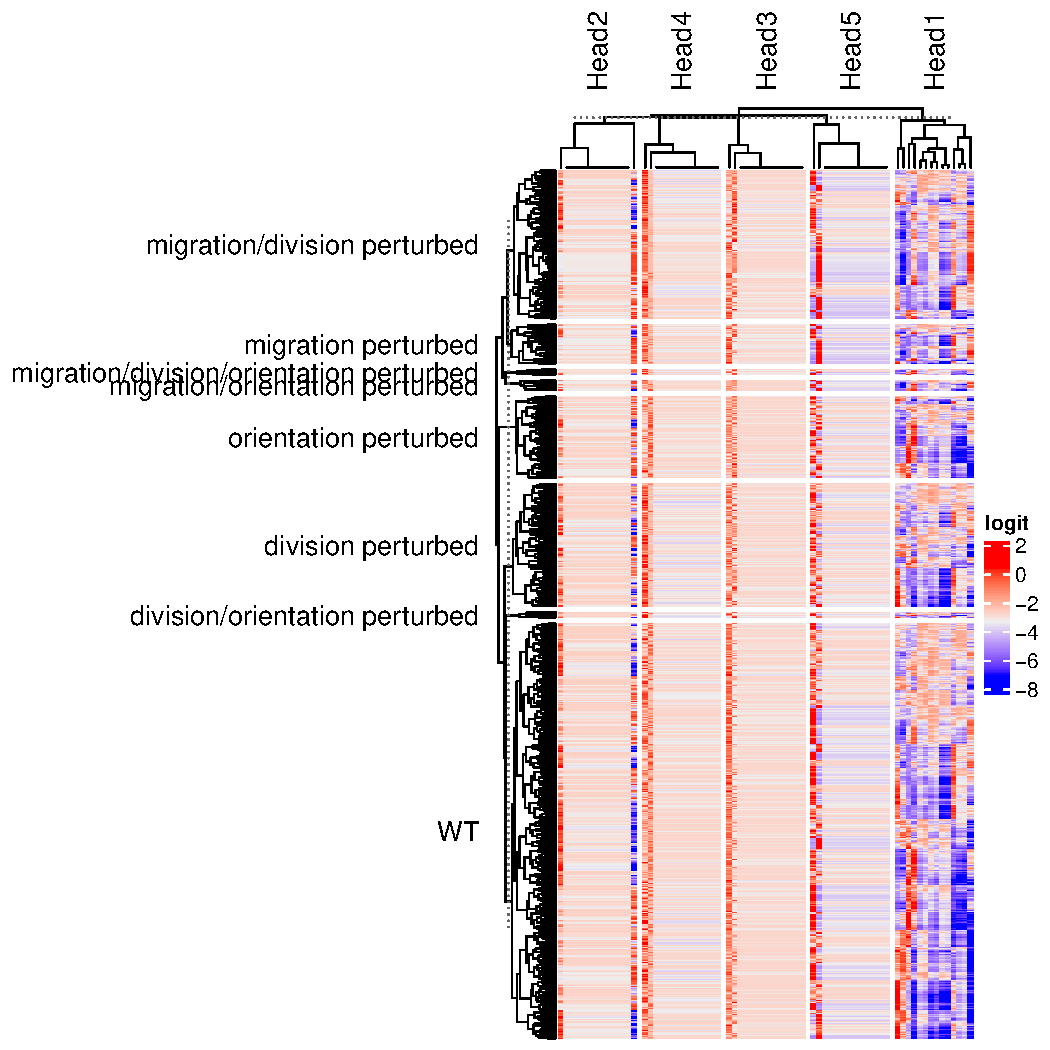
\includegraphics[width=\textwidth]{logits.pdf}
  \caption{For most heads, two clusters dominate.}
  \label{fig:}
\end{figure}

\begin{figure}
  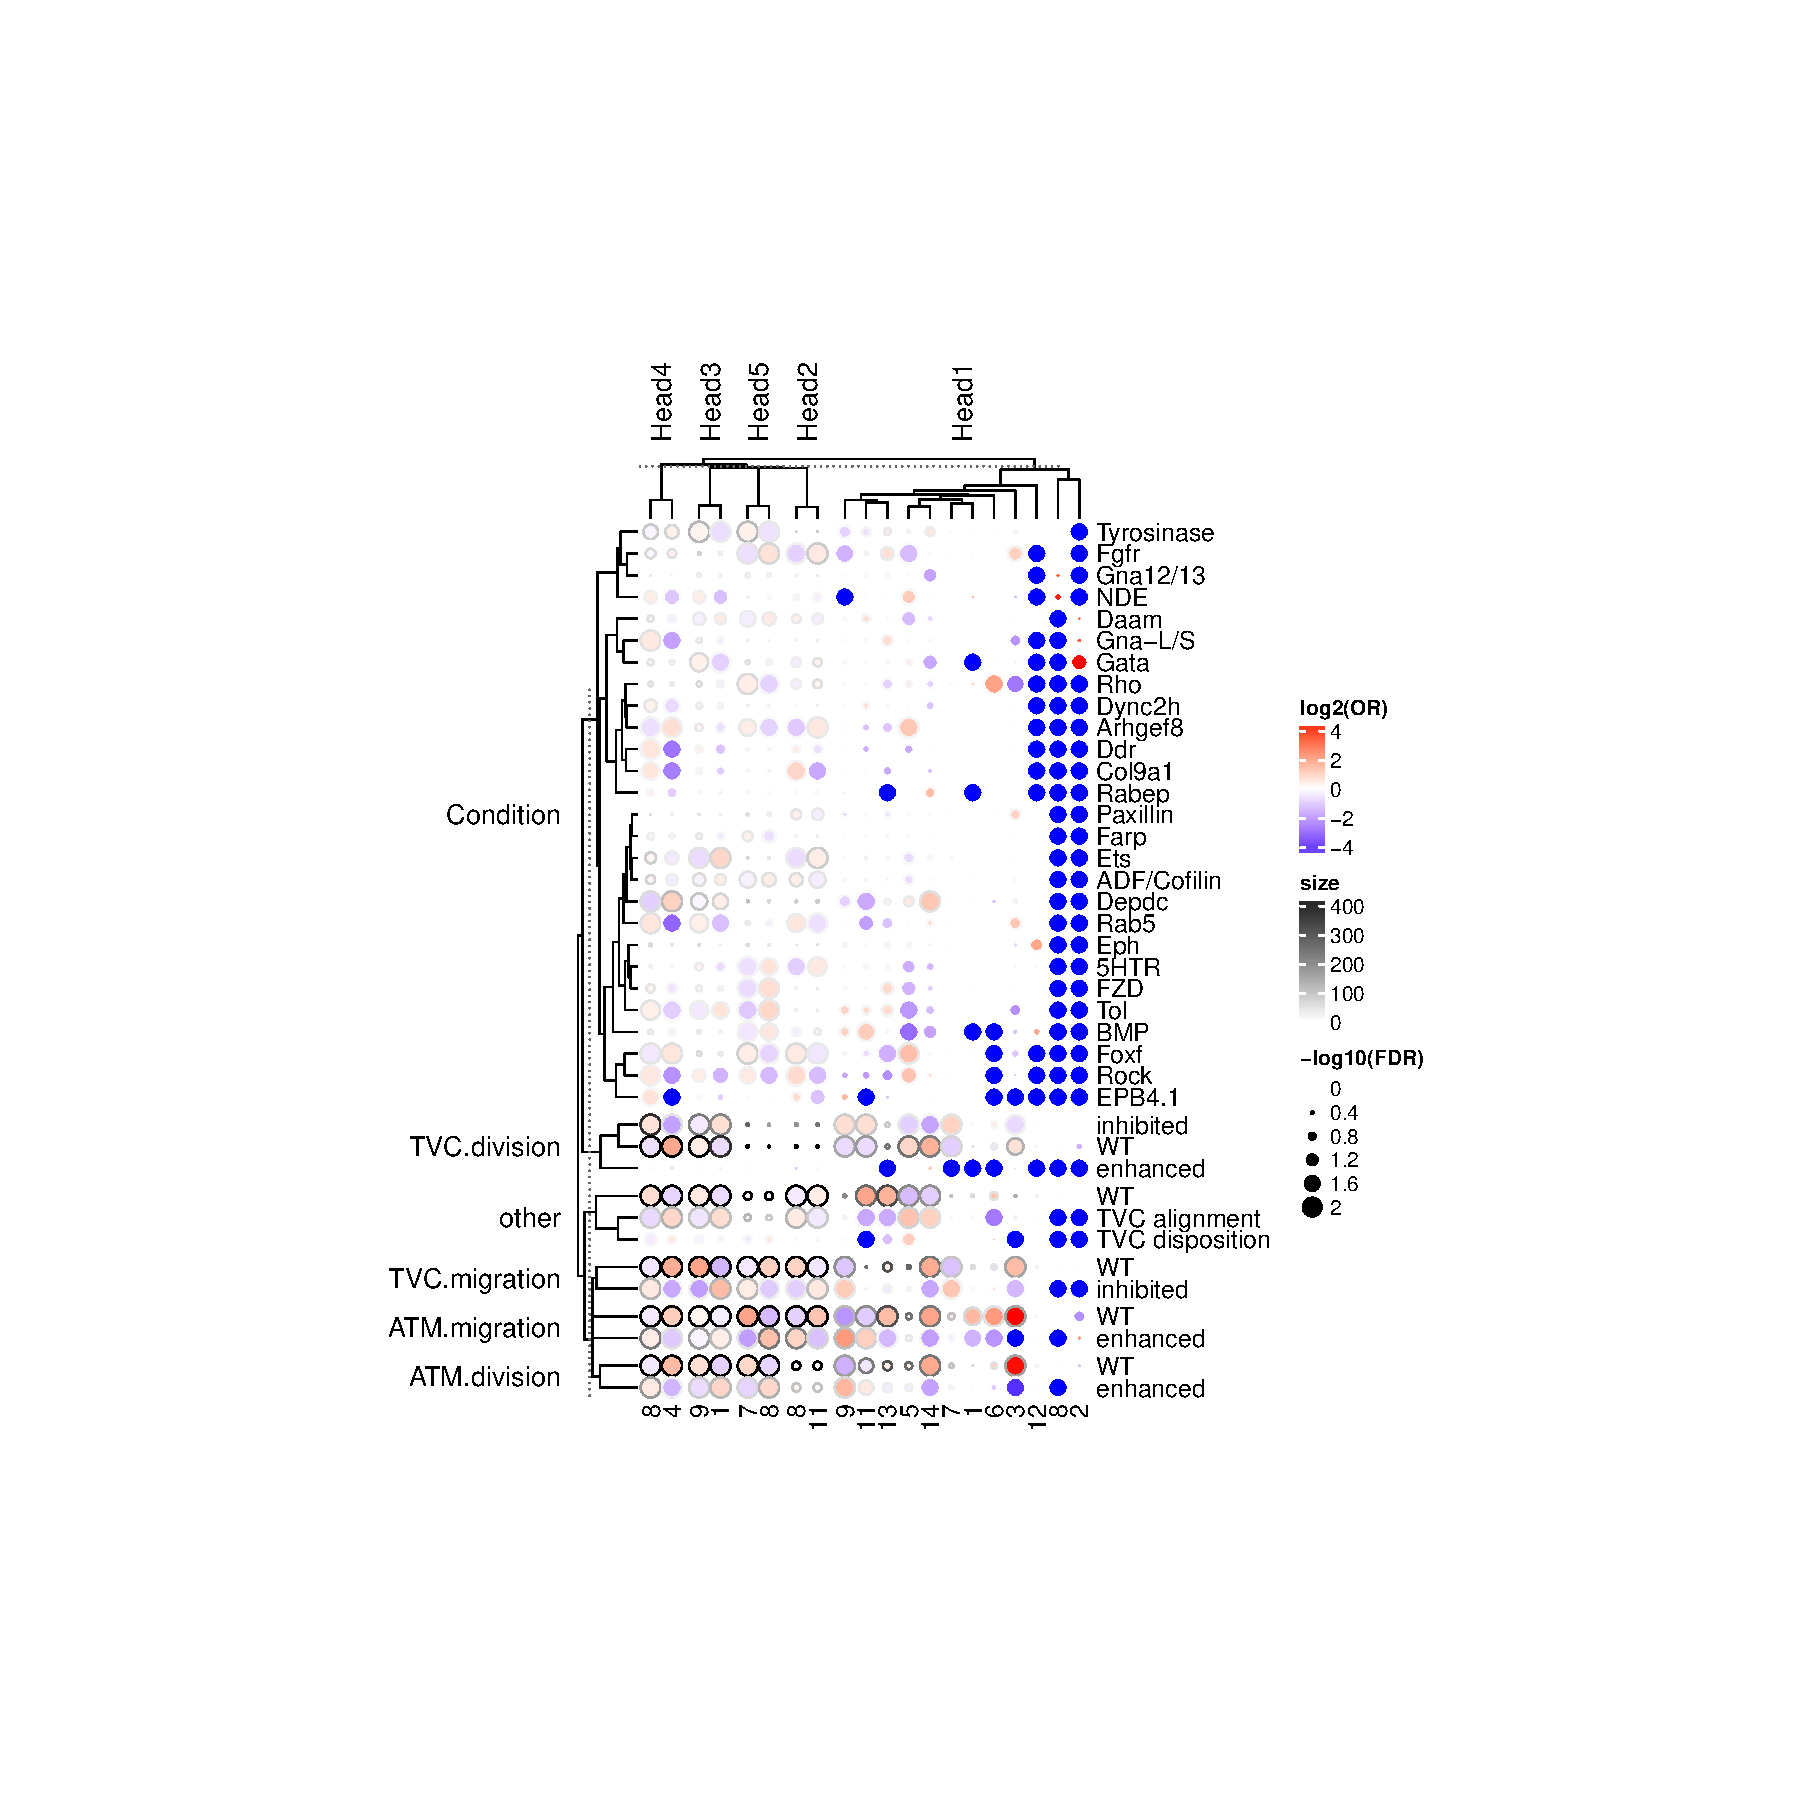
\includegraphics[width=\textwidth]{phenotype.pdf}
  \caption{Hypergeometric test for enrichment of phenotype and treatment condition for each cluster in each head. Dot color indicates overrepresentation of each category in a cluster compared to a uniform prior. Dot size indicates statistical significance of the difference. Dot outline shade indicates number of embryos represented by a dot. Head 1 appears ``polysemantic''. The others appear to distinguish single phenotypic categories.}
  \label{fig:}
\end{figure}
